% !TEX root = ../intro-stellar-physics.tex

\nocite{Mihalas1978Stellar-Atmosph,LeBlanc2010An-Introduction,Carroll2006An-Introduction}

Now that we've discussed radiative transport in the star, we'll explore how the emergent spectrum of a star serves as a diagnostic of ambient conditions in the photosphere.

\section{Overview}

If light from the sun is passed through a grating (a piece of glass with finely etched lines), the light is dispersed in wavelength and creates a spectrum, such as the highly detailed one shown in Fig.~\ref{f.solar-spectrum}. Superposed on the slow variation from red to violet are dark \newterm{absorption lines}. The ions, atoms, and molecules in the solar atmosphere absorb light at specific frequencies and create these lines.
\begin{marginfigure}
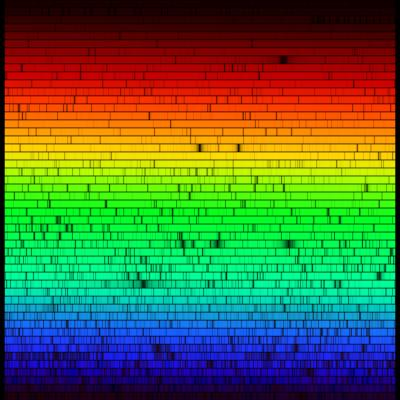
\includegraphics[width=\linewidth]{sunsqa}
\caption[Visible spectrum of the sun]{\label{f.solar-spectrum} Visible spectrum of the sun. Frequency increases along a row from left to right, and by rows from top to bottom. \imgcredcopy\ 
N.A.Sharp (NSF), FTS, NSO, KPNO, NOAO/AURA/NSF.}
\end{marginfigure}

Beginning in the late 1800's, astronomers began classifying stars by the observed absorption lines in the spectra. At this time, Edward Pickering and Williamina Fleming of the Harvard College Observatory began amassing a vast catalog of stellar spectra. They classified these spectra according to the strength of observed hydrogen Balmer lines (the first four are H$\alpha$: \val{657}{\nano\meter}; H$\beta$: \val{486}{\nano\meter}; H$\gamma$: \val{434}{\nano\meter}; H$\delta$: \val{410}{\nano\meter}). Stars, such as Vega, with the strongest Balmer lines were classified as type ``A'', those with the next strongest were type ``B'', and so forth. Annie Jump Cannon, who would later succeed Fleming as curator of astronomical photography at the observatory, simplified and reorganized the scheme, and added decimal subdivisions ($0\ldots9$) for each type\sidenote{For example, the sun's type is G2}. When stellar color is taken into account, the ordering of stars, from blue to red, is ``OBAFGKM''. 

The classification of large numbers of stars allowed for comparison of brightness and spectral type for stars in clusters (and hence at the same distance).
Hertzsprung and Russell independently noticed\cite{Hertzsprung1909Uber-die-Sterne,Russell1914Relations-Betwe} that most stars tended to lie along a band, termed the \newterm{main sequence}, in a plot of absolute magnitude (or luminosity) against stellar type (now known as a \newterm{Hertzsprung-Russell diagram}). Figure~\ref{f.HR} shows some standard main-sequence stars, along with their stellar type and approximate color. The classification of stars based on spectra was put on a firm physical foundation with the influential PhD thesis of Cecilia Payne-Gaposhkin\cite{Payne1925Stellar-Atmosph}, who applied the Boltzmann and Saha equations to show that different stellar spectra were consistent with changes in temperature, rather than composition, of the stellar photosphere. The sequence of stellar types is therefore a temperature sequence, with ``O'' stars being the hottest. 
\begin{marginfigure}
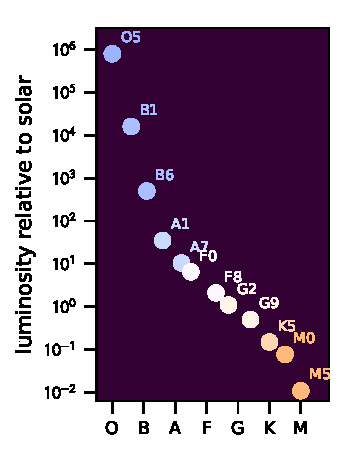
\includegraphics[width=\linewidth]{HR}
\caption[Hertzsprung-Russell diagram of standard main-sequence stars]{\label{f.HR} Hertzsprung-Russell diagram showing standard main-sequence stars. Colors are approximate translations of the spectra.}
\end{marginfigure}

In the 1990's the ``L'' and ``T'' classes were added\cite{Kirkpatrick1999Dwarfs-Cooler-t} for cool stars and brown dwarfs (stellar-like objects that do not reach central temperature sufficient for fusion of hydrogen into helium). With the introduction of the ``Y'' stellar type\cite{Cushing2011The-Discovery-o}, this classification was further extended to even cooler objects having $\Teff\lesssim\val{500}{\K}$.

\section{The hydrogen atom}

To understand why the Balmer lines are strongest in a certain range of temperatures, we first need to review the workings of a hydrogen atom.

The electrons bound to an atom or molecule can only occupy states having a discrete set of energies. For example, the electron in a hydrogen atom only has energies
\begin{equation}\label{e.H-levels}
        E_{n} = -\val{13.6}{\eV}\times \frac{1}{n^{2}},
\end{equation}
where $n > 0$ is an integer known as the \newterm{principal quantum number}.  These energies are negative, relative to a free electron.  For example, the ground state ($n=1$) has energy $-\ERy = -\val{13.6}{\eV}$, meaning that \val{13.6}{\eV} is required to remove an electron in its ground state from the atom.

Because the electrons in an atom can only have certain energies, the atom can only absorb or emit light at specific wavelengths, such that the energy of the photon matches the difference in energy between two levels. For example, a hydrogen atom in its ground state can absorb a photon of energy
\[
        E_{1\to2} = -\ERy \left(\frac{1}{2^{2}} - \frac{1}{1^{2}}\right)
                 = \val{10.2}{\eV}
\]
corresponding to the energy required to excite the electron from level $n=1$ to $n=2$. The wavelengths that can be absorbed by a hydrogen atom at rest can be found by substituting $E = hc/\lambda$ into equation~(\ref{e.H-levels}):
\begin{equation}
        \lambda_{m\to n} = \lambda_{0}\left(\frac{1}{m^{2}}-\frac{1}{n^{2}}\right)^{-1},
\end{equation}
where $\lambda_{0} = \val{91.2}{\nano\meter}$ and $n > m$.
The transitions from the lowest levels are named after their discoverers: Lyman for $1\to n$, Balmer for $2\to n$, Paschen for $3\to n$. A greek letter is used to denote the higher state: for example Lyman $\alpha$ (abbr.\ Ly$\alpha$) means $1\to2$, with $\lambda_{\mathrm{Ly}\alpha} = \val{121.6}{\nano\meter}$. Note that $\lambda_{m\to n} > \lambda_{0}$; photons with wavelengths $\lambda < \val{91.2}{\nano\meter}$ have sufficient energy to knock the electron out of the atom, thereby producing a hydrogen ion and a free electron. The first line transition in the Balmer series is $2\to3$, and is designated H$\alpha$: $\lambda_{\mathrm{H}\alpha} = \val{656.3}{\nano\meter}$. The first 20 lines for each of the Lyman, Balmer, and Paschen series are shown in Fig.~\ref{f.H-spectrum}; note the $3\to4$ transition is outside the plot range. The Balmer lines lie in the visible range.

\begin{marginfigure}
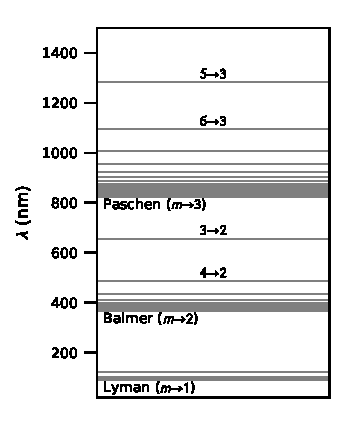
\includegraphics[width=\linewidth]{H-spectrum}
\caption{Spectral lines of neutral hydrogen 
\label{f.H-spectrum}}
\end{marginfigure}

\section{The Boltzmann Equation}
\label{s.boltzmann-eqn}

In order to produce a Balmer absorption line, we must have some hydrogen atoms in the photosphere with electrons in the energy level $n=2$. The more atoms in a state $n=2$, the more absorption and the stronger the line. To find the number of atoms with energy level $n=2$, we make use of a fundamental result, due to Boltzmann, from statistical (thermal) physics; namely, that if our sample of atoms is in thermal equilibrium, then the ratio of the number of atoms with energy $E_{i}$ to the number of atoms with energy $E_{j}$ is
\begin{equation}\label{e.boltzmann}
\frac{N_{i}}{N_{j}} = \frac{g_{i}}{g_{j}} 
\exp\left(-\frac{E_{i}-E_{j}}{\kB T}\right).
\end{equation}
Here the number $g_{n}$ gives the number\sidenote{$g_{n}$ is known as the \emph{degeneracy} of a given level $n$} of quantum mechanical states having energy $E_{n} = -\ERy/n^{2}$. For an energy level $n$, there are $n^{2}$ possible states, each having a different angular momentum. For each of these $n^{2}$ states, both the electron and proton may each have 2 possible spins. The total number of states for energy $E_{n}$ is therefore $g_{n} = 2\times2\times n^{2}$.

Suppose we wish to know the fraction of atoms in a given state $i$: that is, we wish to know
\[	x_{i} = \frac{N_{i}}{N_{1}+N_{2}+\ldots+N_{i}+\ldots} . \]
Using equation~(\ref{e.boltzmann}), we can express $x_{i}$ as 
\begin{eqnarray}
  x_{i} &=& \frac{g_{i}e^{-E_{i}/\kB T}}{g_{1}e^{-E_{1}/\kB T}+g_{2}e^{-E_{2}/\kB T}+\ldots+g_{i}e^{-E_{i}/\kB T}+\ldots} \nonumber\\
        &\equiv& \frac{g_{i}e^{-E_{i}/\kB T}}{\pfcn},
\end{eqnarray}
where the quantity 
\begin{equation}\label{e.partition-function}
	\pfcn = \sum_{n} g_{n}\exp\left(-\frac{E_{n}}{\kB T}\right)
\end{equation}
is the \emph{partition function}. Loosely speaking, the partition function indicates the number of ways the sample of atoms can be partitioned among the different energy levels.

\begin{sidebar}[The partition function for neutral hydrogen]
\label{sb.partition-function}
The partition function for neutral hydrogen, eq.~(\ref{e.partition-function}), diverges as $n\to\infty$. To see this, substitute $g_{n}=4n^{2}$ and $E_{n} = -\ERy/n^{2}$ and factor out common terms to obtain
\[	\pfcn = 4e^{\beta\ERy}\sum_{n} n^{2} e^{-\beta\ERy(1-1/n^{2})}, \]
with $\beta = (\kB T)^{-1}$. The sum evidently diverges, since for $n\gg 1$ the individual terms approach $n^{2}e^{-\beta\ERy}$. In practice, this divergence isn't a problem, as there is an upper limit on $n$ set by ambient conditions. For example, the mean distance of the electron from the nucleus is $\approx \abohr n^{2}$, where $\abohr = \val{\sci{5.29}{-11}}{\cm}$ is the Bohr radius. As a result, each atom takes up a volume $\approx \abohr^{3}n^{6}$; if the atoms are not to overlap, then the volume per atom, $V/N \equiv 1/\xi$, must be larger than this by some factor. To make this concrete, set the volume of an atom to be less than half of that available in our gas:
\[
\abohr^{3}n^{6} \lesssim \frac{1}{2}\frac{V}{N} = \frac{1}{2\xi}.
\]
Thus the maximum level is $n < (2\abohr^{3}\xi)^{-1/6}$. For a typical A-star photospheric density $\xi\sim \val{10^{15}}{\cm^{-3}}$, the energy level cutoff is $n \approx 35$. In practice the cutoff will be even lower because of collisions.

You might worry that this estimate for the maximum value of $n$ is a bit sloppy. Fortunately,
the precise maximum value of $n$ is unimportant for most applications. The reason is that the terms in the partition function increase only slowly. As an example, the terms and cumulative sum in the partition function at a temperature $T=\val{10^{4}}{\K}$ are as follows.
\begin{center}
\begin{tabular}{rrr}
$n$ & $n^{2} e^{-\beta\ERy(1-1/n^{2})}$ & $4\sum_{i=1}^{n} i^{2}e^{-\beta\ERy(1-1/i^{2})}$ \\
\hline
   1 & 1.00e+00 &  4.0000 \\
   2 & 2.88e-05 &  4.0001 \\
   3 & 7.23e-06 &  4.0001 \\
  \multicolumn{3}{c}{\vdots} \\
  26 & 9.62e-05 &  4.0038 \\
  \multicolumn{3}{c}{\vdots} \\
  52 & 3.78e-04 &  4.0274 \\
  \multicolumn{3}{c}{\vdots} \\
 268 & 9.99e-03 &  7.5901 \\
\end{tabular}
\end{center}
As we can see from the cumulative sum (rightmost column), the value of the partition function is insensitive to cutoff until $n$ is quite large; indeed, for many applications it is reasonably accurate to just use $Q\approx 4e^{\beta\ERy}$. 
\end{sidebar}

\begin{exercisebox}[Partition function for neutral hydrogen]
Assuming that the first term $g_{1}e^{-E_{1}/\kB T}$ dominates the sum in the partition function (see Box~\ref{sb.partition-function}), plot the fraction of neutral hydrogen in its $n=2$ state as a function of temperature, for $\val{5\,000}{\K} < T < \val{20\,000}{\K}$.
\end{exercisebox}

\section{Ionization: The Saha equation}
\label{s.saha-eqn}

As the temperature in the gas rises, there are more photons with sufficient energy to eject electrons from an atom. In addition, collisions between atoms also become sufficiently energetic to ionize the atom. In astronomical nomenclature, the ionization state is denoted by a small Roman numeral: \ion{Fe}{i} denotes neutral iron, \ion{Fe}{ii} denotes singly-ionized iron (charge $+1$), \ion{Fe}{iii} denotes doubly-ionized iron (charge $+2$), and so on. In thermal equilibrium, the rate at which atoms are ionized must equal the rate at which ions and electrons recombine: for example, in a gas consisting of hydrogen atoms, hydrogen ions (i.e., protons), and electrons the reaction
\[
	\ion{H}{ii} + e \longleftrightarrow \ion{H}{i}
\]
is in equilibrium. We'd like to extend equation~(\ref{e.boltzmann}) to find the ratio of two ionization states $N_{i+1}/N_{i}$. Although deriving this equation, termed the \newterm{Saha equation}\sidenote{Derived by Meghnad Saha in 1920}, is beyond the scope of the course, what we shall do is take the equation apart and try to understand how it works.  The Saha equation for the ratio of the populations of two ionization states
\sidenote{In this context, $N_{i+1}/N_{i}$ refers to ratios such as $N_{\ion{Fe}{ii}}/N_{\ion{Fe}{i}}$. Each population $N$ can be divided into sub-populations based on the different electron energy levels. For example, $N_{\ion{H}{i}} = N_{\ion{H}{i},1} + N_{\ion{H}{i},2} + \ldots$, where $N_{\ion{H}{i},2}$ are the number of hydrogen in ionization state I with an electron in the second energy level.}
$N_{i+1}$ and $N_{i}$ is
\begin{equation}\label{e.saha}
\frac{N_{i+1}}{N_{i}} 
= {\color{red}\left[\frac{2}{n_{e}}
\left(\frac{m_{e}\kB T}{2\pi\hbar^{2}}\right)^{3/2}\right]}
{\color{blue}\frac{\pfcn_{i+1}}{\pfcn_{i}}}.
\end{equation}
In this equation, $n_{e}$ denotes the electron density---the number of free electrons per unit volume---and $m_{e}$ is the electron mass. The terms $\pfcn_{i+1}$ and $\pfcn_{i}$ are the partition functions for the two states, \emph{both measured with respect to the same zero-point for energy}. To understand better what this equations means, let's consider each of the color-coded factors in turn.

Start with the term $\color{blue} Q_{i+1}/Q_{i}$. If both partition functions are dominated by the ground state term\sidenote{see Box~\ref{sb.partition-function}} then
\begin{eqnarray*}
	\frac{Q_{i+1}}{Q_{i}} &=& \frac{g_{i+1,1}}{g_{i,1}} e^{-\beta (E_{i+1,1}-E_{i,1})}\\
	&=& \frac{g_{i+1,1}}{g_{i,1}} e^{-\beta\,E_{\mathrm{ion}}}
\end{eqnarray*}
Here $E_{\mathrm{ion}} = E_{i+1,1} - E_{i,1}$ is the energy needed to remove an electron from an ion in state $i$ and we use the common shorthand $\beta = (\kB T)^{-1}$. Thus $Q_{i+1}/Q_{i}$ resembles the Boltzmann equation~(\ref{e.boltzmann}).

The additional factor in $\color{red}\left[\cdot\right]$ in eq.~(\ref{e.saha}) arises because we also need to allow for the number of free electron states. When the atom is ionized, each electron quickly acquires an average kinetic energy $(3/2)\kB T$. There are many different states having this energy: the electron can be in different locations and moving in different directions, for example.  

You might think that there would be an infinitude of possible electron states.  Quantum mechanics, however, sets limitations on this number. First, we have the Pauli exclusion principle: no two electrons can be in the same location with the same momentum and same spin. What do we mean by same location and momentum?  Recall the Heisenberg uncertainty principle: the electrons $x$-position and $x$-momentum are spread about a range of values $\Delta x$ and $\Delta p_{x}$, and these uncertainties are related via
\[ \Delta x\,\Delta p_{x} \gtrsim h. \]
Thus, if we imagine dividing our volume into little boxes of volume
\[ 
 \Delta V = \Delta x\,\Delta y\,\Delta z \approx \frac{h^{3}}{\Delta p_{x}\,\Delta p_{y}\,\Delta p_{z}},
\]
each box can hold two electrons.\sidenote{Because electrons have spin 1/2, we can put two electrons into the same position and momentum state if their spins are oppositely directed.} Suppose we have a volume $V$; how many boxes are there?  The number of available boxes is
\[
	\frac{V}{\Delta V} \approx \frac{V\;\Delta p_{x}\,\Delta p_{y}\,\Delta p_{z}}{h^{3}}.
\]
To estimate the size of $\Delta p_{x}\,\Delta p_{y}\,\Delta p_{z}$, let's take $\Delta p_{x}\sim p_{x}$ and similarly for $\Delta p_{y}$ and $\Delta p_{z}$; further, if everything is isotropic then $p_{x}\approx p_{y}\approx p_{z}$ on average, so $\Delta p_{x}\,\Delta p_{y}\,\Delta p_{z} \sim p_{x}^{3}$.  Now the kinetic energy of the electron is $p^{2}/2m_{e}$, and $p^{2} = p_{x}^{2} + p_{y}^{2} + p_{z}^{2} \approx 3 p_{x}^{2}$. Hence the kinetic energy is $(3/2)p_{x}^{2}/m_{e}$; in thermal equilibrium, however, the kinetic energy has an average value of $(3/2)\kB T$.  The value of $p_{x}^{2}$ is therefore
\[
	p_{x}^{2} \approx m_{e}\kB T,
\]
and the number of boxes is
\[
	\frac{V}{\Delta V} \sim V\frac{p_{x}^{3}}{h^{3}} \sim V\frac{\left(m_{e}\kB T\right)^{3/2}}{h^{3}}.
\]
If our volume $V$ contains $N_{e}$ electrons, then the number of states electron is
\[
	\frac{2V}{N_{e}\Delta V} \sim \frac{2V}{N_{e}}\frac{\left(m_{e}\kB T\right)^{3/2}}{h^{3}}.
\]
The factor of 2 appears because each box can hold 2 electrons.  Recognizing that $N_{e}/V = n_{e}$, we see that this number of states per free electrons corresponds to the factor in $\color{red}\left[\cdot\right]$ in equation~(\ref{e.saha}). When the numerical calculation is done correctly, the additional factor of $2\pi$ arises.

The number of states per free electron plays an important role in setting the temperature at which a species ionizes. You might expect, since a term $e^{-E_{\mathrm{ion}}/\kB T}$ appears in the ratio $N_{i+1}/N_{i}$, that a species would ionize at a temperature $E_{\mathrm{ion}}/\kB$. In fact the ionization temperature is much lower. To see how this works, define
\[
	\zeta = \ln\left[\frac{1}{n_{e}}\left(\frac{m_{e}\kB T}{2\pi\hbar^{2}}\right)^{3/2}\right].
\]
We can then write eq.~(\ref{e.saha})---with the approximation that the partition functions are dominated by the ground state---as
\[
	\frac{N_{i+1}}{N_{i}} = \frac{2g_{i+1,1}}{g_{i,1}}\exp\left(\zeta - \beta E_{\mathrm{ion}}\right).
\]
Now the factor $g_{i+1,1}/g_{i,1}$ is of order unity. Hence, when the gas ionizes and $N_{i+1,1}\approx N_{i,1}$, we must have that $\zeta\approx \beta E_{\mathrm{ion}}$; put differently, the ionization temperature will not be $E_{\mathrm{ion}}/\kB$ but rather $E_{\mathrm{ion}}/\kB\zeta$. Under conditions in the photosphere of an A star ($T \approx \val{10^{4}}{\K}$, $n\sim \val{10^{15}}{\cm^{-3}}$), $\zeta \approx 15$.

In more intuitive terms, when an electron is ejected from an atom, it has an enormously large number $\sim e^{15}$ number of different states available. To rejoin with an ion requires being in the right place at the right time with the right energy. The large number of available states makes this unlikely, so the electron must wander lonely through a vast and desolate phase space until at long last it reunites with an ion. In a sense, the large number of available states per electron makes ionization easier than recombination; as a result the temperature at which ionization occurs is considerably lower than $E_{\mathrm{ion}}/\kB$.

\begin{exercisebox}[Conditions for strong Balmer lines]
\label{ex.strong-Balmer}
Let $n_{\textsc{i}}$ be the density of \ion{H}{i} and $n_{\textsc{ii}}$ be the density of \ion{H}{ii}. Denote the fraction of neutral hydrogen as $x = n_{\textsc{i}}/(n_{\textsc{i}}+n_{\textsc{ii}})$, so that $1-x = n_{\textsc{ii}}/(n_{\textsc{i}}+n_{\textsc{ii}})$ is the fraction of ionized hydrogen. Take $n_{\textsc{i}}+n_{\textsc{ii}} = \val{10^{15}}{\cm^{-3}}$, and assume that all free electrons come from the ionization of hydrogen, so that $n_{e} = n_{\textsc{ii}}$. Plot $x$ as a function of temperature for $\val{7\,500}{\K}\le T\le \val{15\,000}{\K}$, and find the temperature at which $x = 1/2$. Then multiply $x$ by the fraction $n_{2}/n_{1}$, as set by the Boltzmann equation, to find the fraction of hydrogen in the $n=2$ level.
\end{exercisebox}

As shown in exercise~\ref{ex.strong-Balmer}, the Balmer lines, which correspond to transitions $2\to3$, $2\to 4$, \ldots, are most prominent in A stars. These stars have $\Teff = \valrng[--]{7\,500}{9\,500}{\K}$. At lower temperatures, the population of hydrogen atoms in the level $n=2$ decreases as $e^{-E_{2}/\kB T}$ and the lines become weak. At higher temperatures, the number of neutral hydrogen atoms decreases; most of the hydrogen is ionized, and the Balmer lines again become weaker.

These arguments apply to other species present in the stellar photosphere. Figure \ref{f.spectral-types} displays spectra for selected stellar types at optical wavelengths. In the hottest stars (type O: $\Teff > \val{30\,000}{\K}$), hydrogen is mostly ionized and the lines are from \ion{He}{ii} and multiply-ionized metals. As the temperature cools into the B and A series, the hydrogen lines increase in strength. Going from F into G ($\Teff = \valrng[--]{5\,000}{6\,000}{\K}$), the hydrogen lines decrease, while lines from singly-ionized and neutral metals such as \ion{Ca}{ii}, \ion{Ca}{i}, and \ion{Fe}{i} become strong.  At still lower temperatures in the K and M ($\Teff < \val{3\,500}{\K}$) types, absorption from molecules such as TiO becomes prominant.  An example is the broad trough seen in the K spectrum near $\lambda = \val{500}{\nano\meter}$.

\begin{figure}[hbp]
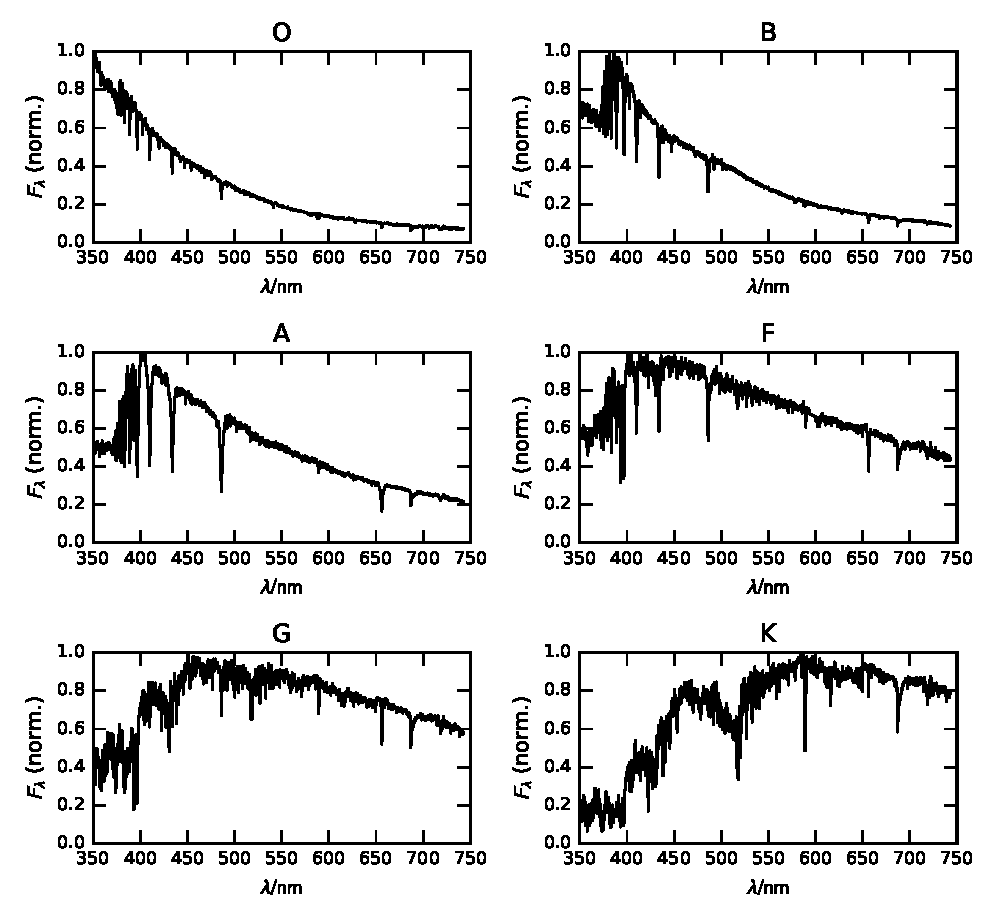
\includegraphics[width=\linewidth]{spectral_types}
\caption[Standard stellar types]{\label{f.spectral-types} Spectra from main-sequence stars of spectral types O--K. Data from \protect\citet{Jacoby1984A-library-of-st}.}
\end{figure}

\section{Pressure broadening of lines}

We've now demonstrated how stars may be classified by the absorption lines in their spectra, and how this classification gives us the photosphere effective temperature. We can also obtain information about the pressure at the photosphere, and hence the surface gravity of the star, by looking at the shape of the absorption lines. A zoomed-in view of the H$\gamma$ line ($2\to5$ transition in \ion{H}{i}) from a main-sequence A1 star is show in Fig.~\ref{f.single-line}. The line is spread over a few nanometers, compared against a central value of $\val{434}{\nano\meter}$.
\begin{marginfigure}[-8\baselineskip]
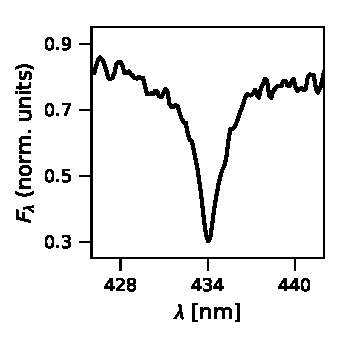
\includegraphics[width=\linewidth]{single-line}
\caption[H$\gamma$ absorption line]{\label{f.single-line} H$\gamma$ absorption line observed from the main-sequence A1 star HD16608. Spectrum from \protect\citet{Jacoby1984A-library-of-st}.}
\end{marginfigure}

\newthought{To understand what sets the shape, and width, of the absorption line,} we need to model our atomic transition. Consider an electronic transition in an atom between two energy levels, $E_m$ and $E_n$. The natural frequency of this transition is $\nu_0 = |E_n-E_m|/h$. Light incident on the atom with frequency $\nu\neq\nu_0$ drives the electron at frequency $\nu$. 

Since the transition between two states has a definite frequency associated with it, let's start with a simple harmonic oscillator, which is described by an equation
\[
	\DDtt{x} + \omega_{0}^{2} x = 0.
\]
Here $\omega_{0} = 2\pi\nu_{0}$. Light is described as an electromagnetic wave, so classically the electron feels a force $eE\cos(\wt)$, where $\omega = 2\pi \nu$. An accelerating electron radiates, which damps the acceleration of the electron. The damping can be modeled as a force that is proportional to the velocity, $-m\Gamma \dif x/\dif t$. Classically, the transition in an atom can therefore be modeled as an electromagnetic oscillator with damping and driving terms,
\[
	\DDtt{x} + m\Gamma\DDt{x} + \omega_{0}^{2}x = \frac{eE}{m}\cos(\wt).
\]
This has a well known solution (see Box~\ref{sb.damped-driven-oscillator}). The amplitude of oscillation is proportional to the energy removed from the incident light, which is proportional to the cross-section. The classical cross-section for absorption of radiant energy by an electromagnetic oscillator is thus
\begin{equation}\label{e.semi-classical}
    \sigma = \left(\frac{\pi e^2}{m_e c}\right)
    \left\{\frac{\Gamma/4\pi}{(\nu_0-\nu)^2 + (\Gamma/4\pi)^2}\right\}.
\end{equation}
\begin{marginfigure}
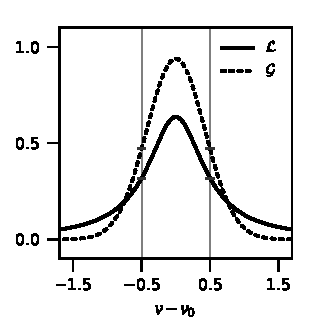
\includegraphics[width=\linewidth]{comparison}
\caption[Comparison of Lorentzian and Gaussian distributions]{\label{f.comparison}
Comparison of a Lorentzian ($\mathcal{L}$, solid line) and a Gaussian ($\mathcal{G}$, dotted line), both with $\mathrm{FWHM}=1$. The area under each curve is unity.}
\end{marginfigure}
The function
\[
    \mathcal{L}(\nu;\Gamma) = \frac{1}{\pi} 
        \frac{\Gamma/4\pi}{(\nu_0-\nu)^2 + (\Gamma/4\pi)^2}
\]
is known as a \newterm{Lorentzian}.  In contrast to a Gaussian, a Lorentzian is characterized by broad ``wings'' (Fig.~\ref{f.comparison}) away from the central frequency $\nu_{0}$.
The actual value of the cross-section must be calculated using quantum mechanics. The overall shape of the cross-section is still in the form of equation~(\ref{e.semi-classical}), however, so the opacity is just
\begin{equation}
    \rho\kappa_\nu = n_{\mathrm{ion},m} \left(\frac{\pi e^2}{m_e c}\right) f_{mn}
        \left\{\frac{\Gamma/4\pi}{(\nu_0-\nu)^2 + (\Gamma/4\pi)^2}\right\}.
\end{equation}
In this equation, $f_{mn}$ is a number, called the \emph{oscillator strength}, that results from the calculation of the transition probability from state $m$ to state $n$, and $n_{\mathrm{ion},m}$ is the density of atoms in state $m$.  The key point is that $f_{mn}$ depends only on the details of the transition: the energies, spins, and parities of the atomic states.  It does not depend on environmental parameters such as temperature and pressure.  As a result, $f_{mn}$ can be measured or computed once and then tabulated.

\begin{sidebar}[The driven damped oscillator]
\label{sb.damped-driven-oscillator}
Let's begin with a simple system: a mass $m$ attached to a spring with force $F = -kx$.

\begin{center}
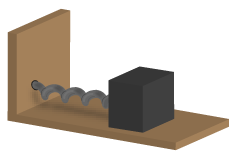
\includegraphics[width=0.5\linewidth]{simple-spring}
\end{center}

\noindent If we put the origin of our coordinate system where the mass is at rest with the spring relaxed, then the equation of motion of the mass is
\begin{equation}\label{e.SHO-basic}
	\DDtt{x} + \frac{k}{m} x = 0.
\end{equation}
You have solved this equation before: the most general solution is
\begin{equation}\label{e.SHO-general-solution}
	x(t) = x_{0}\cos(\wot) + \frac{v_{0}}{\omega_{0}}\sin(\wot)
\end{equation}
with $\omega_{0}^{2} = k/m$ and with $x_{0}$ and $v_{0}$ being the initial position and velocity of the mass. The angular frequency $\omega_{0}$ is related to the period of oscillation $T$ as $\omega_{0} = 2\pi/T = 2\pi\nu$.

\newthought{Now let's push on our mass with an oscillating force, $F\cos(\omega t)$ with $\omega\neq\omega_{0}$.} A real world example would be holding a vibrating tuning fork near another fork tuned to a different frequency.  The equation of motion is now
\begin{equation}\label{e.SHO-driven}
	\DDtt{x} + \omega_{0}^{2}x = \frac{F}{m}\cos(\wt).
\end{equation}
You can verify by substitution that a general solution is
\[
	x(t) = \frac{F/m}{(\omega_{0}^{2}-\omega^{2})}\cos(\wt) + A\cos(\wot)+B\sin(\wot).
\]
Let's start with our harmonic oscillator at rest ($v_{0} = \left.\dif x/\dif t\right|_{t=0} = 0$) and at $\left. x\right|_{t=0} = 0$.  With these conditions, we can determine the constants $A$ and $B$; the solution is
\[
	x(t) = \frac{F/m}{(\omega_{0}^{2}-\omega^{2})}\left[\cos(\wt)-\cos(\wot)\right].
\]
Let's recast this by defining $\Delta = \omega_{0} - \omega$ and $\omega_{m} = (\omega_{0}+\omega)/2$.  Then
\begin{eqnarray*}
  \omega_{0}^{2}-\omega^{2} &=& (\omega_{0}-\omega)(\omega_{0}+\omega) = 2\Delta\omega_{m},\\
  \cos(\wot) &=& \cos\left(\wmt+\Delta t/2\right),\\
  \cos(\wt) &=& \cos\left(\wmt-\Delta t/2\right);
\end{eqnarray*}
using the cosine addition rules and combining terms, we can write the solution as
\begin{equation}\label{e.beats}
	x(t) = {\color{red}\left[\frac{F/m}{\Delta\omega_{m}}\sin(\Delta t/2)\right]}{\color{blue}\sin(\wmt)}.
\end{equation}
This illustrates the phenomena of \newterm{beats}: the oscillation consists of a \textcolor{blue}{carrier signal} at frequency $\omega_{m}$ with the \textcolor{red}{amplitude} modulated at the slower frequency $\Delta /2$.  Notice that the amplitude increases as $\Delta \to0$, i.e., $\omega\to\omega_{0}$.

\newthought{Now let's make our model even more realistic.}
We add a frictional force that is proportional to velocity, $F_{\mathrm{friction}} = -m\Gamma \dif x/\dif t$. Our complete equation of motion is then
\begin{equation}
	\DDtt{x} + \Gamma \DDt{x} + \omega_{0}^{2}x = \frac{F}{m}\cos(\omega t).
\end{equation}
The solution to this is straightforward to find, although the algebra is tedious (trust me on this). The general solution for initial conditions $\left.x\right|_{t=0} = x_{0}$ and $\left.\dif x/\dif t\right|_{t=0} = v_{0}$ is
\begin{eqnarray}
\label{e.general-solution-ddo}
\lefteqn{x(t) = \frac{F\womw/m}{\womw^{2}+\gw}\cos(\omega t)} && \\
	&+& \frac{\Gamma\omega F/m}{\womw^{2}+\gw}\sin(\omega t)\nonumber \\
	&+& {\color{SlateGrey}\left[x_{0}-\frac{F\womw/m}{\womw^{2}+\gw}\right] e^{-\Gamma t/2} \cos(\omega_{\Gamma}t)} \nonumber\\
	&+& {\color{SlateGrey}\left[\frac{v_{0}}{\omega_{\Gamma}}-\frac{\Gamma\omega F/m}{\womw^{2}+\gw}
	\,\frac{\omega}{\omega_{\Gamma}}\right]e^{-\Gamma t/2} \sin(\omega_{\Gamma}t)}, 
	\nonumber
\end{eqnarray}
with
\[ 
    \omega_{\Gamma} = 
        \omega_{0}\left(1-\frac{\Gamma^{2}}{4\omega_{0}^{2}}\right)^{1/2}.
\]
Let's simplify this a bit.  First, the last two terms decay as $e^{-\Gamma t/2}$: these are transients set by the initial conditions. After a time $t \gg 2/\Gamma$, therefore, only the first two terms, which oscillate at the driving frequency $\omega$, will remain. 

We can simplify these first two terms even further: if we write
\[ \cos(\wt) = \frac{e^{i\wt}+e^{-i\wt}}{2},\quad \sin(\wt) 
    = \frac{e^{i\wt}-e^{-i\wt}}{2i}, \]
we can combine them and obtain
\begin{eqnarray}
    x(t) &=& \frac{F}{2m}\left[\frac{1}{\left(\omega_0^2-\omega^2\right) + i\Gamma\omega}\right]e^{i\wt} \nonumber\\
    && + \frac{F}{2m}\left[\frac{1}{\left(\omega_0^2-\omega^2\right) - i\Gamma\omega}\right]e^{-i\wt} \nonumber\\
    &=& \Re\left\{\frac{F}{m}\left[\frac{1}{\left(\omega_0^2-\omega^2\right) + i\Gamma\omega}\right]e^{i\wt}\right\}.\label{e.oscillator-expression}
\end{eqnarray}
We use the symbol ``$\Re$'' to denote taking the real part of a complex quantity.
The oscillation is thus described as the real part of a complex quantity $Ae^{i\wt}$, with
\[
    A = \frac{F}{m}\left[\frac{1}{\left(\omega_0^2-\omega^2\right) + i\Gamma\omega}\right]
\]
being the (complex) amplitude.

For $\omega \approx \omega_0$, we approximate $(\omega_0^2-\omega^2)\approx 2\omega_0(\omega_0-\omega)$ and take the square of the amplitude to find,
\begin{eqnarray}
    \left|A\right|^2 &=& \left(\frac{F}{2m\omega_0}\right)^2
        \frac{1}{(\omega_0-\omega)^2 + (\Gamma/2)^2}\nonumber\\
    &=& \frac{\pi}{2\Gamma}\left(\frac{F}{m\omega_0}\right)^2
        \left\{\frac{1}{\pi}\frac{\Gamma/2}{(\omega_0-\omega)^2 + (\Gamma/2)^2}\right\}
\end{eqnarray}
We rewrote the amplitude in the second line so that the term in $\{\cdot\}$ is normalized; in fact, it is the Lorentzian function $\mathcal{L}(\omega;\Gamma)$ in terms of the driving frequency $\omega$.
\end{sidebar} 

\newthought{In a stellar atmosphere, the width $\Gamma$ is set by collisions.} For example, when an electron passes close by our atom, the electric field shifts the energy levels of the atom\sidenote{This is an application of the \emph{Stark} effect that you learn about in quantum mechanics.}.  The greater the collision rate, the larger the width.
If we have two stars of the same photospheric temperature (so that both stars have the same lines), then a way to increase the collision rate is to increase the pressure. Recall, however, that in the stellar atmosphere $P = (g/\kappa)\tau$; as a result, stars with a higher surface gravity will have broader lines. The inset in Figure~\ref{f.compare_grav} illustrates the broadening of the Balmer H$\gamma$ line ($2\to5$) in the spectrum of a main-sequence A1 star compared with that of a supergiant A1 star.

\begin{figure}[hp]
\forcerectofloat
    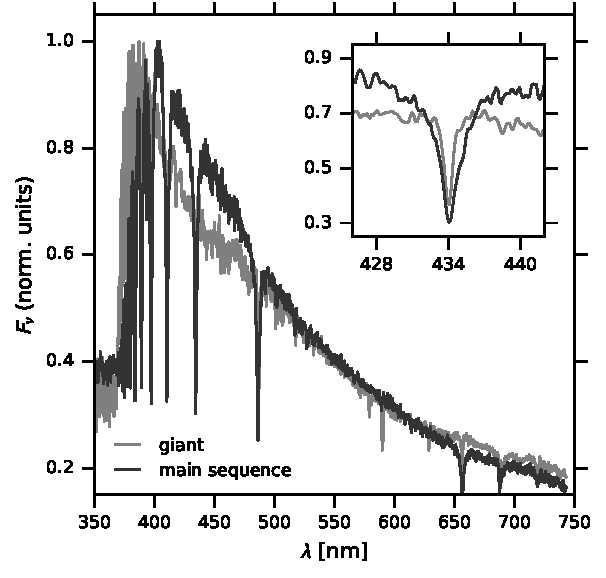
\includegraphics[width=\linewidth]{compare_grav}
    \caption[Spectra of two A1 stars]{\label{f.compare_grav}
    Spectra of two A1 stars, HD 16608 (a main sequence star) and SAO 12149 (a supergiant star).  Spectra are from \citet{Jacoby1984A-library-of-st}.
    }
\end{figure}
